%!TEX root = main.tex

\section{Application: Arithmetics autograder}
In the application of arithmetics autograder, the input image is ususally very large (typically around \(3000\times2000\) pixels), among which 10\% are black pixels.
This means if we apply ``Algorithm 4'' directly, the input list of coordinates typically have length \(10^5\) to \(10^6\), which is too long for the algorithm to return the results in reasonable period of time.
A more promising approach is to split the procedure into the following steps:
\begin{enumerate}
    \vspace{-0.5em}
    \item cluster the worksheet into equations;
    \vspace{-0.5em}
    \item cluster the numbers and operators in each equation from step 1.
\end{enumerate}


\subsection{Equation clustering}
One observation is that step 1 does not need accuracy in the numbers and operators, so that we can resample the input image so that the input for Algorithm 4 is significantly reduced (to around \(10^3\) coordinates of black pixels).
\begin{figure}[htbp]
    \vspace{-1em}
    \centering
    \begin{subfigure}[t]{0.45\textwidth}
        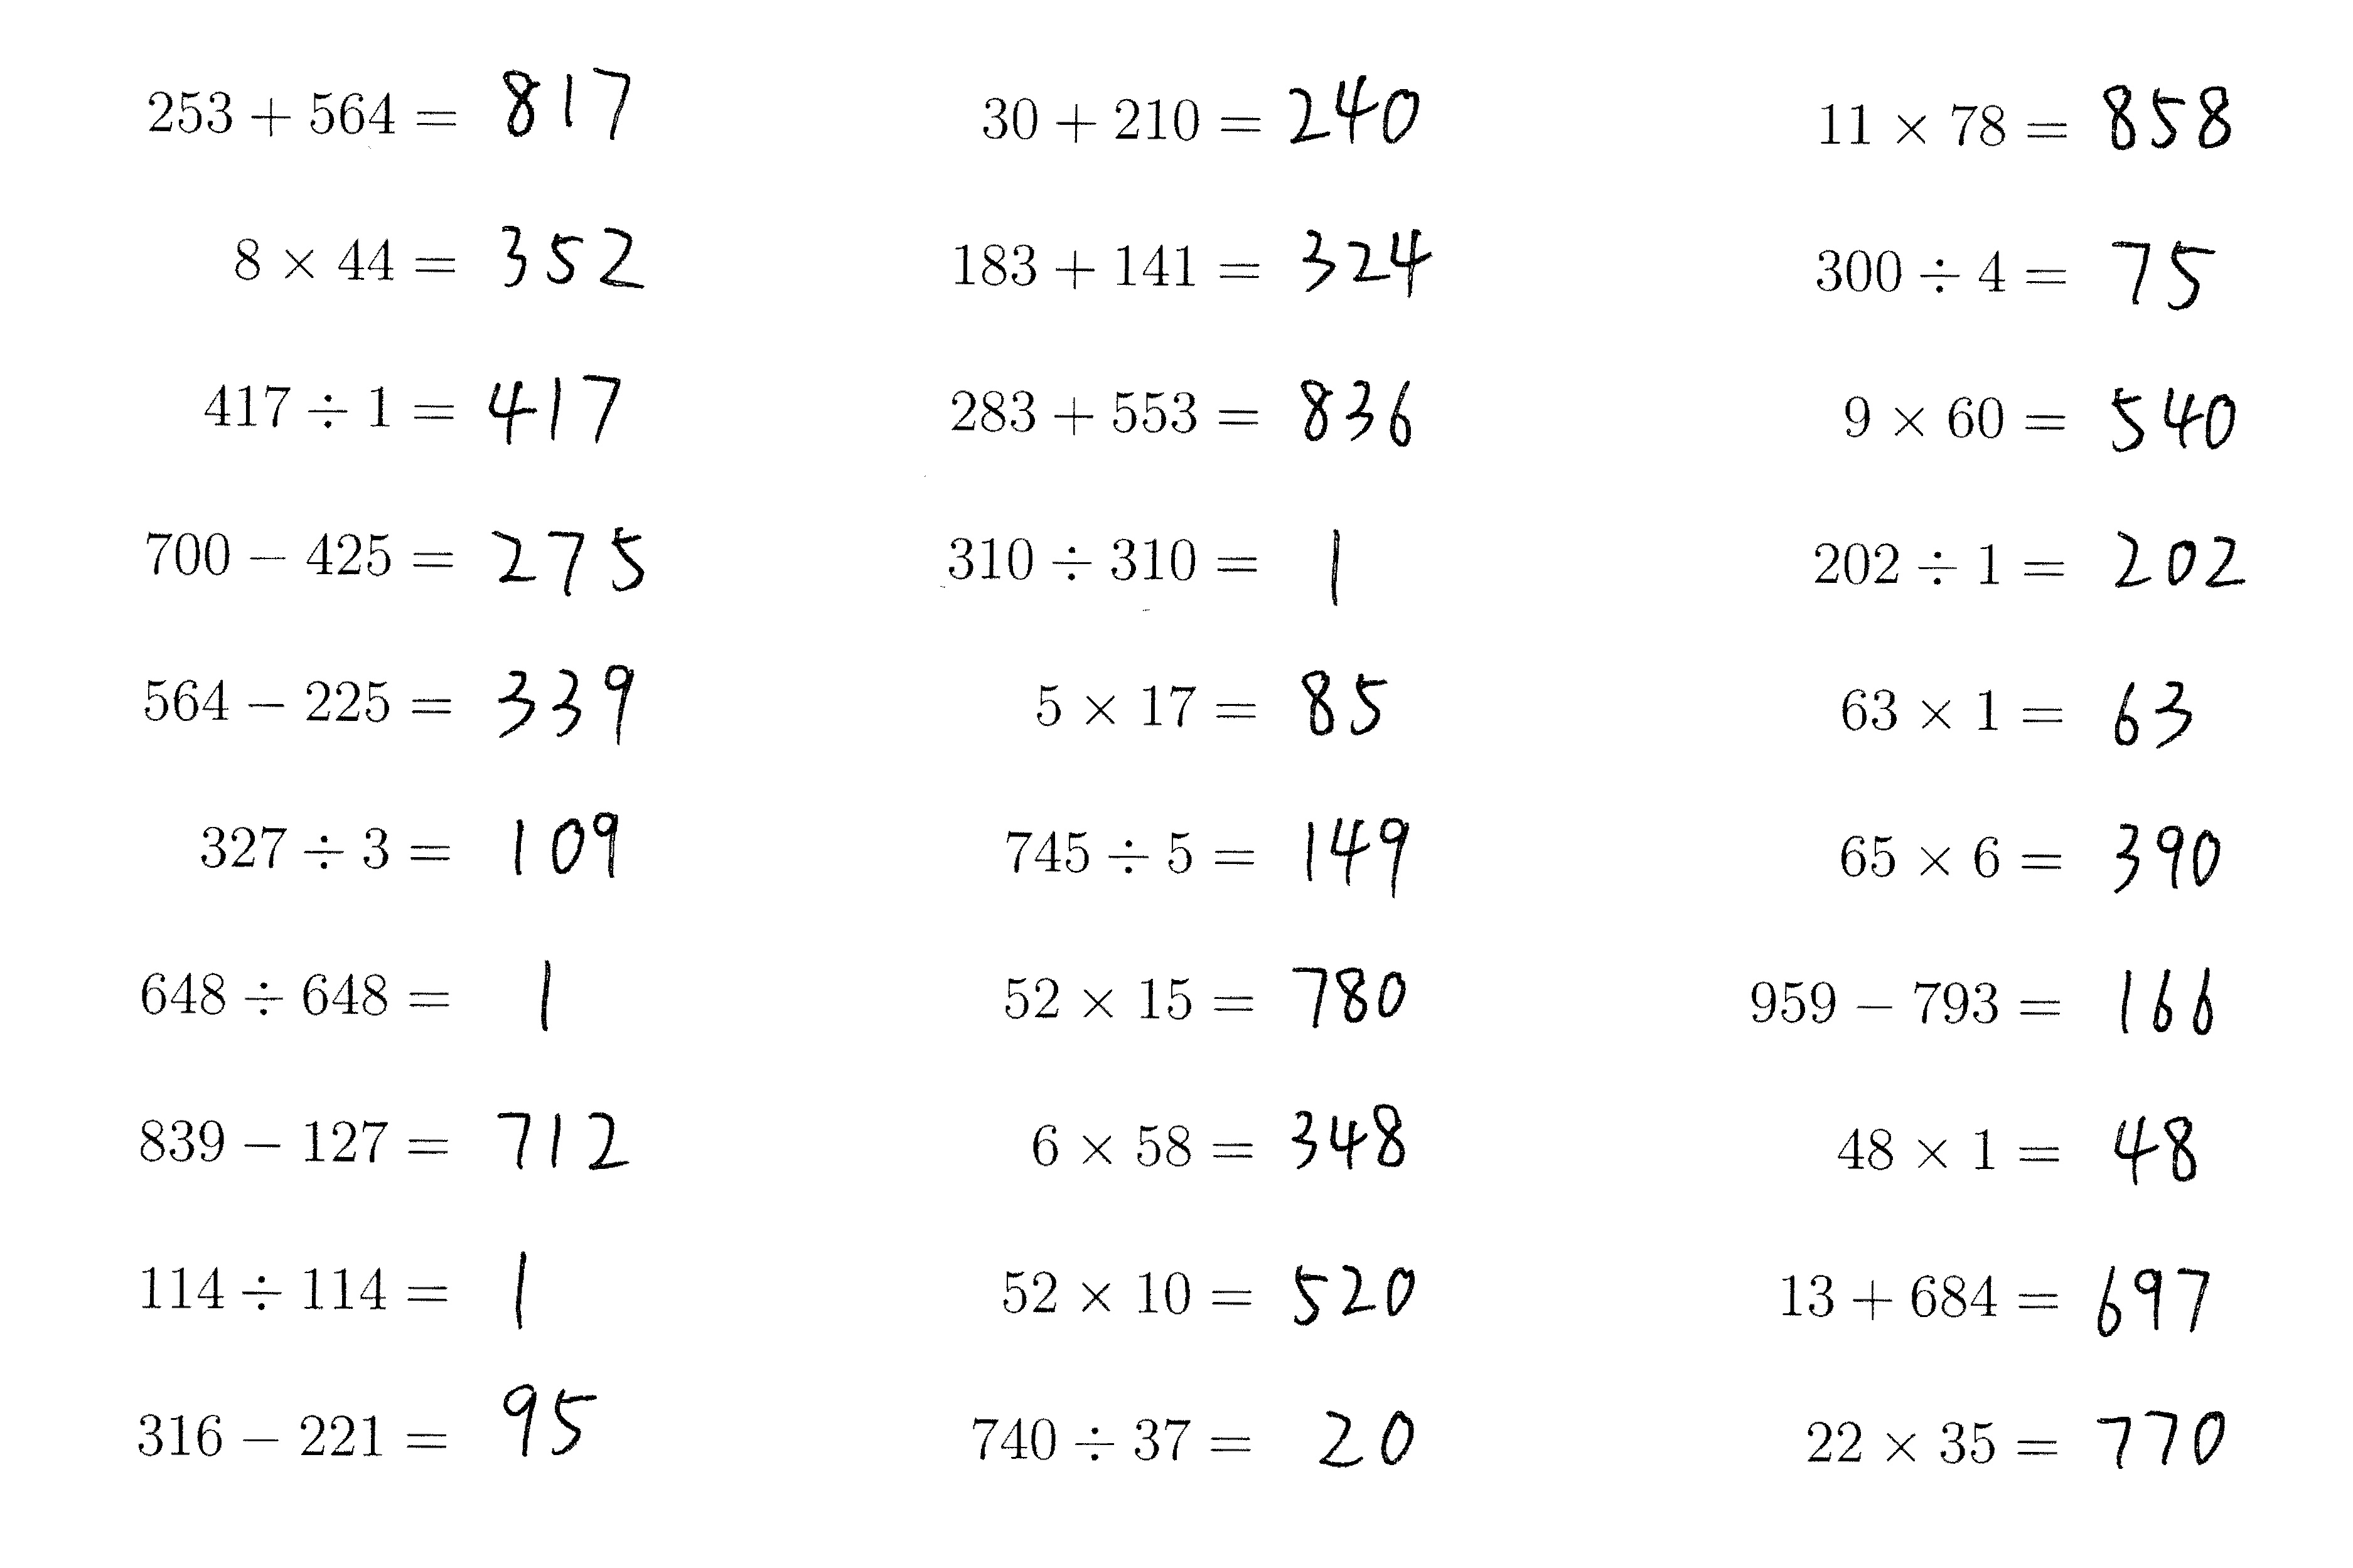
\includegraphics[width=\textwidth]{../TestSamplePictures/test1.png}
        \caption{Input image}\label{fig10a}		
    \end{subfigure}
    \begin{subfigure}[t]{0.54\textwidth}
        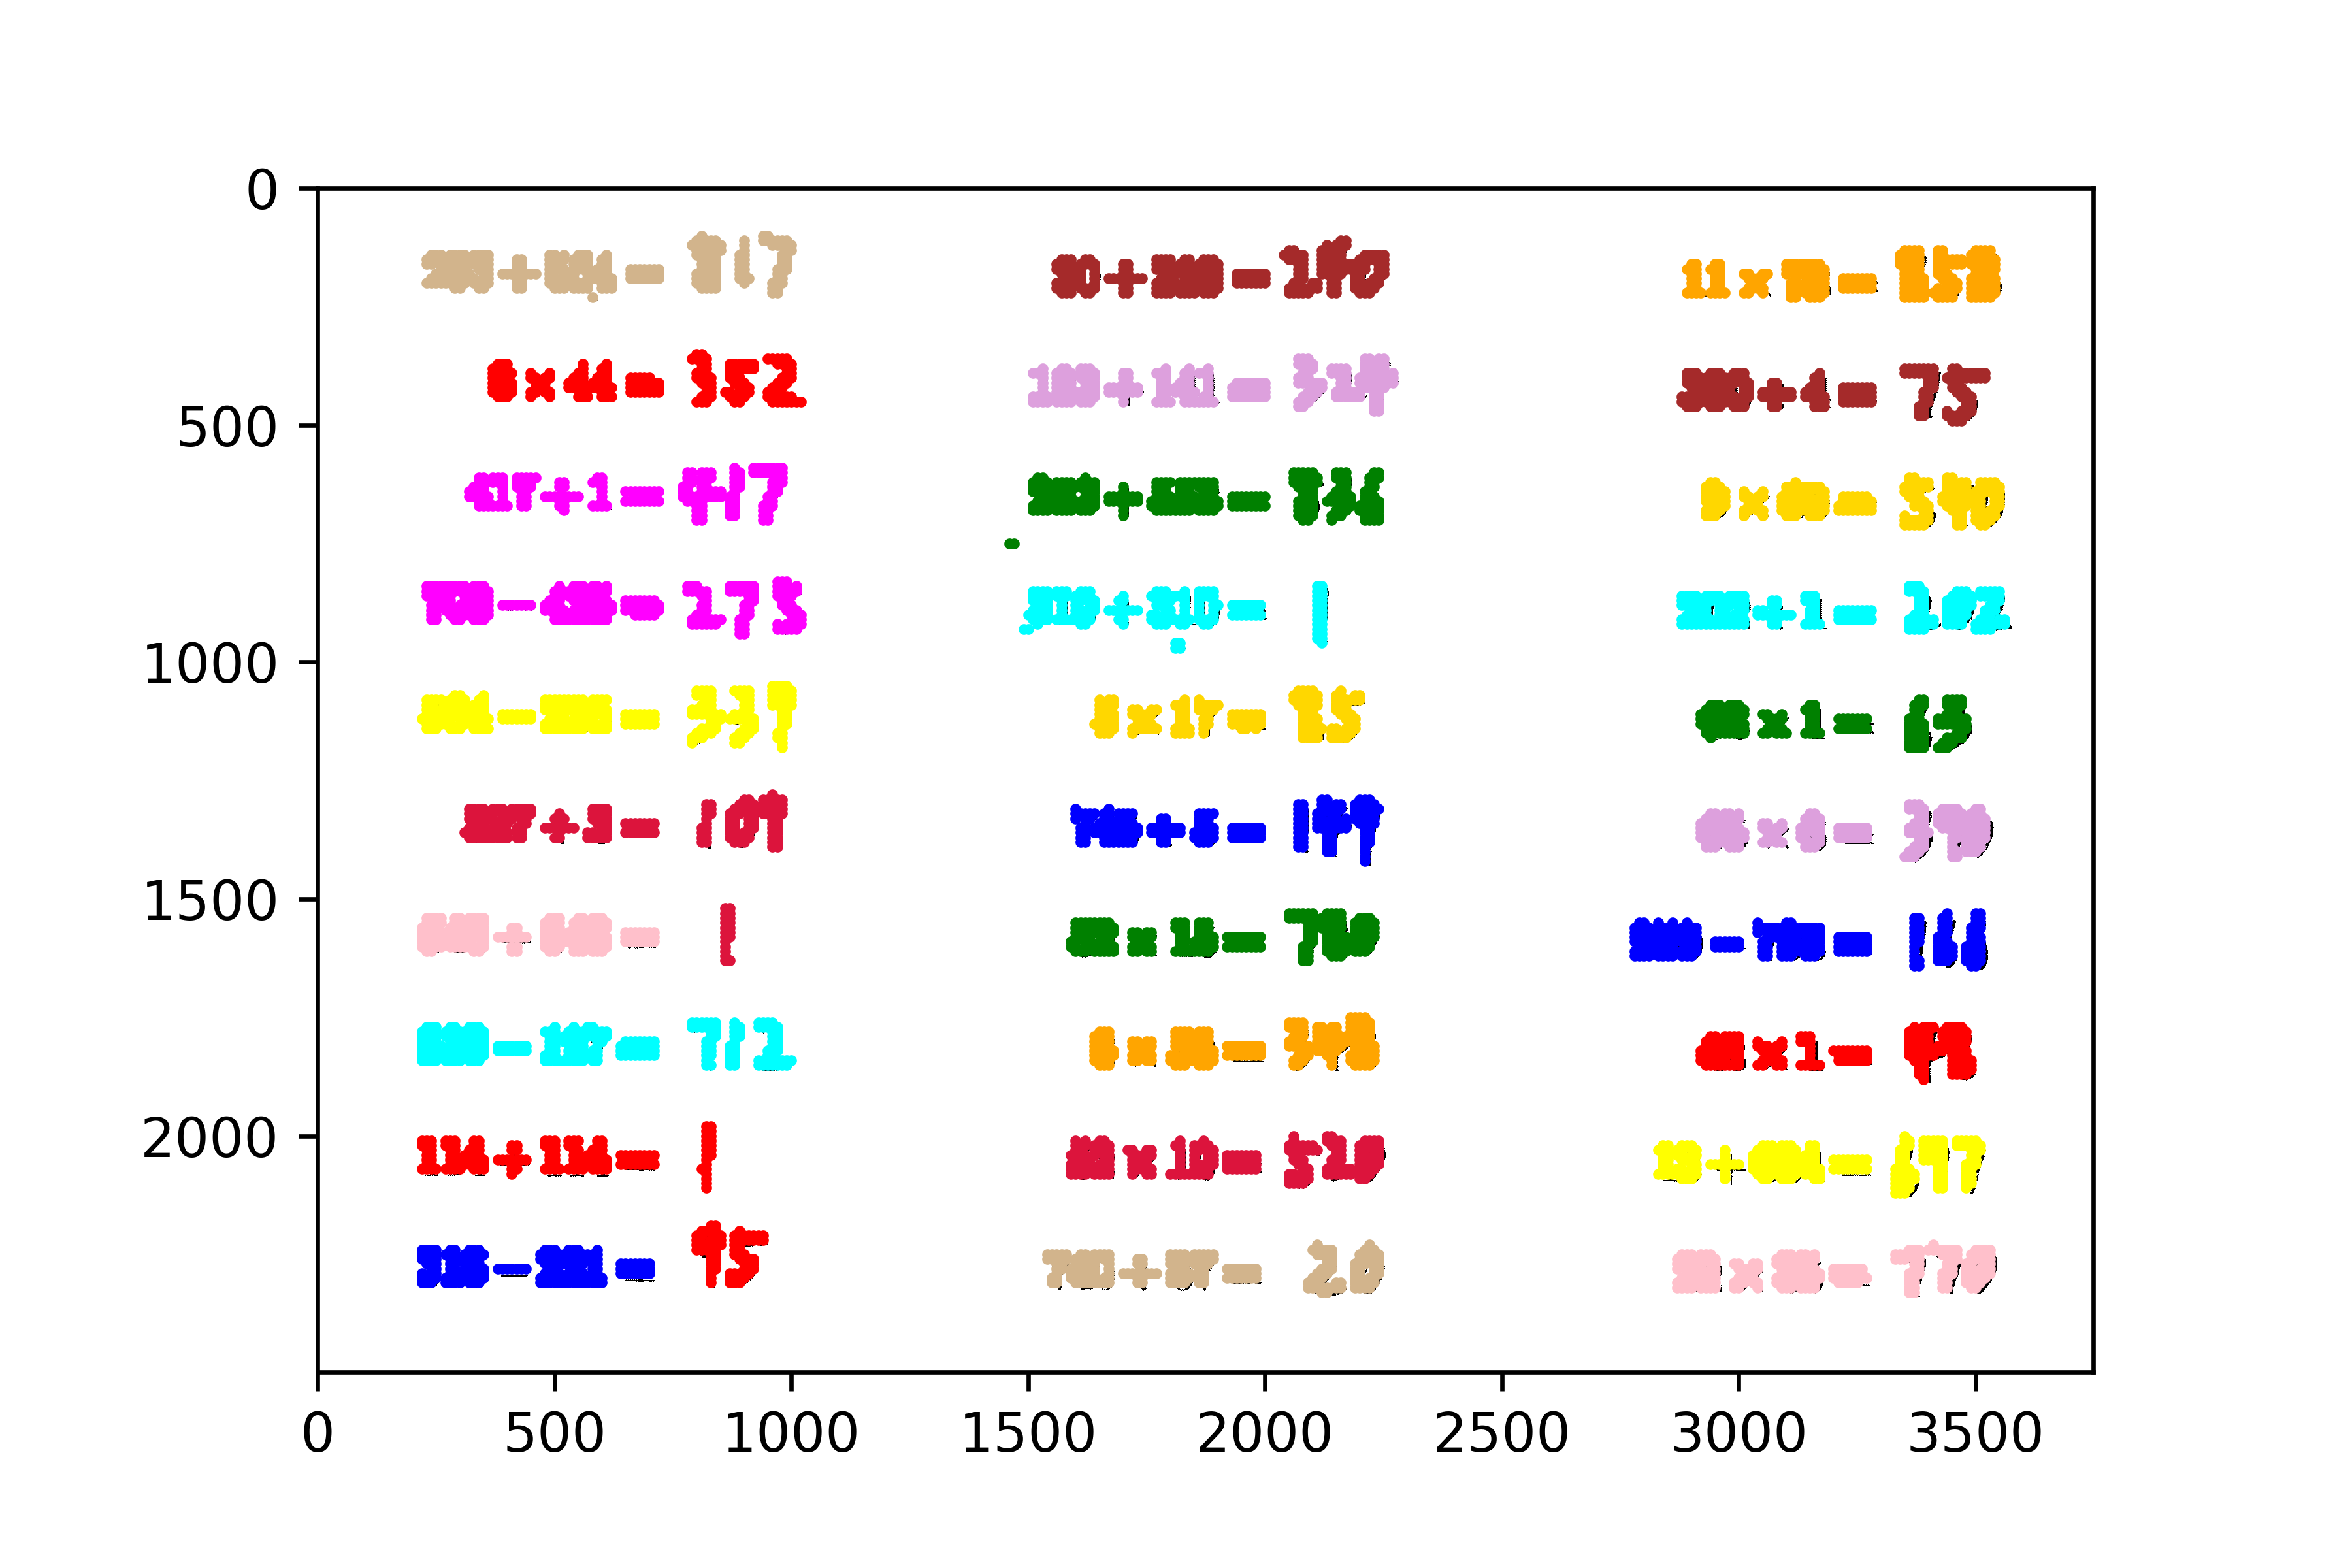
\includegraphics[width=\textwidth]{../TestSamplePictures/test1_result.png}
        \caption{Equation clustering effect}\label{fig10b}
    \end{subfigure}
    \caption{Equation clustering by Algorithm 4}\label{fig10}
\end{figure}
We can see from \autoref{fig10b} is blurred compared with the input \autoref{fig10a}, and most of the equations are correctly clustered.

\subsection{Numbers and operators clustering}
By the result of step 1, we can crop the equations from original input with high resolution and apply Algorithm 4 again.
\begin{figure}[htbp]
    \vspace{-1em}
    \centering
    \begin{subfigure}[t]{0.33\textwidth}
        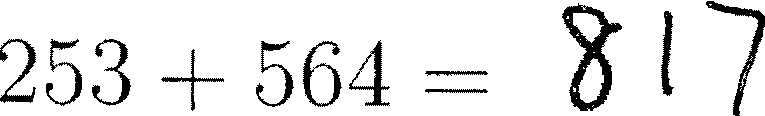
\includegraphics[width=\textwidth]{../TestSamplePictures/test3.png}
        \caption{Input equation 1 from step 1}\label{fig11a}		
    \end{subfigure}
    \begin{subfigure}[t]{0.66\textwidth}
        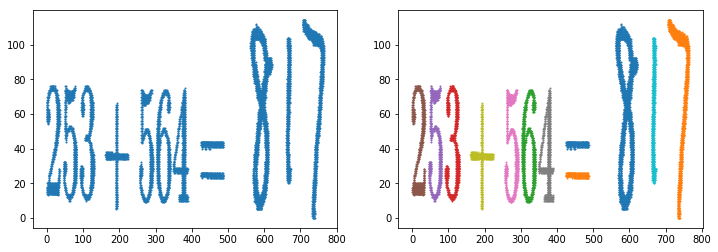
\includegraphics[width=\textwidth,height=0.3in]{../TestSamplePictures/test3_result.png}
        \caption{number \& operators clustering effect on equation 1}\label{fig11b}
    \end{subfigure}
    \begin{subfigure}[t]{0.33\textwidth}
        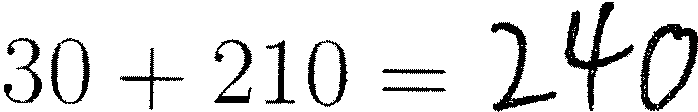
\includegraphics[width=\textwidth]{../TestSamplePictures/test4.png}
        \caption{Input equation 2 from step 1}\label{fig11c}		
    \end{subfigure}
    \begin{subfigure}[t]{0.66\textwidth}
        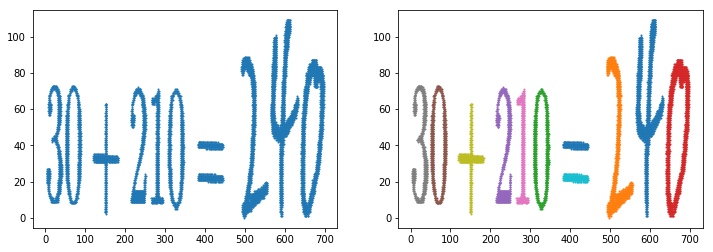
\includegraphics[width=\textwidth,height=0.3in]{../TestSamplePictures/test4_result.png}
        \caption{number \& operators clustering effect on equation 2}\label{fig11d}
    \end{subfigure}
    \begin{subfigure}[t]{0.33\textwidth}
        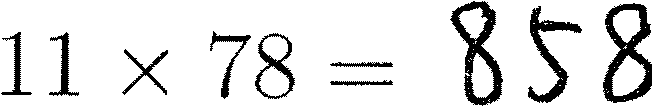
\includegraphics[width=\textwidth]{../TestSamplePictures/test5.png}
        \caption{Input equation 3 from step 1}\label{fig11e}		
    \end{subfigure}
    \begin{subfigure}[t]{0.66\textwidth}
        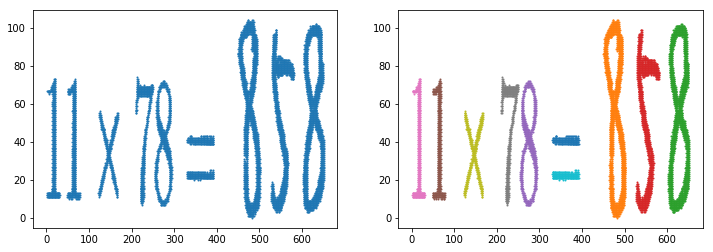
\includegraphics[width=\textwidth,height=0.3in]{../TestSamplePictures/test5_result.png}
        \caption{number \& operators clustering effect on equation 3}\label{fig11f}
    \end{subfigure}
    \caption{Number and operators clustering by Algorithm 4}\label{fig11}
\end{figure}
In real application, we will encounter more intersections that should NOT be separated.
For example, the operators \(+,\times\) and digits 4, 6 and 8 have intersections in their shapes, but if the clustering algorithm separate them apart, the digit classifer will almost surely give a wrong result.
In our test examples, \autoref{fig11b} contains a printed 4 and 6 and a handwritten 8, \autoref{fig11d} contains a handwritten 4 and \autoref{fig11f} contains a printed 8 and two handwritten 8s, all of which are not separated apart, so that they can be correctly recognized by a standard digit classifer.
Also, the \(+\) signs in \autoref{fig11b} and \autoref{fig11d} and the \(\times\) sign in \autoref{fig11f} are all clustered correctly, so they will probably be correctly recognized by an operator classifer.

\subsection{Comparison with existing algorithms}
Phone APPs which autograde student's arithmetics worksheet are available (both iOS and Android platforms) for years.
Based on our test, they can grade our input \autoref{fig10a} 100\% correctly in less than 1 second on iPhone X.
Our autograder based on Algorithm 4 already made some mistakes in step 1, which makes it impossible to compete on correctness with their performance.
Furthermore, the computational complexity of our autograder is also much higher, taking around 30 seconds on step 1 and 5 seconds for each equation on step 2 on PC (Intel i7-8550U).
This means the spectral clustering algorithm is useful in clustering numbers and operators, but is far less than enough to build a robust autograder.
The developers of these APPs made much more assumptions and optimized much more to make it run on mobile devices.